% !TeX program = xelatex
%% METADATA
%% subject-code: DI01000051
%% subject-name: Fundamentals of Electronics
%% semester: 1
%% examination: Summer-2025
%% date: 12-06-2025
%% description: Solution guide for Fundamentals of Electronics
%% tags: study-material, solutions, gtu, DI01000051
%% END METADATA

\documentclass{article}

% content/resources/templates/preamble.tex
\usepackage[margin=0.6in]{geometry}
\author{Milav Dabgar}
\usepackage{amsmath,amssymb,amsthm}
\usepackage{booktabs}
\usepackage{multirow}
\usepackage{xcolor}
\usepackage{tcolorbox}
\tcbuselibrary{breakable,skins}
\usepackage[colorlinks=true,linkcolor=blue]{hyperref}
\usepackage{titlesec}
\usepackage{enumitem}
\usepackage{tikz}
\usepackage{pgfplots}
\usepackage{circuitikz}
\usepackage[version=4]{mhchem}
\usepackage{longtable}
\usepackage{array}
\usepackage{float}
\usepackage{caption}
\usepackage{listings}

\lstset{
  basicstyle=\small\ttfamily,
  breaklines=true,
  breakatwhitespace=false,
  postbreak=\mbox{\textcolor{red}{$\hookrightarrow$}\space},
  float=false,
  numbers=left,
  numberstyle=\tiny\color{gray},
  numbersep=10pt,
  xleftmargin=2em,
  keywordstyle=\color{blue},
  commentstyle=\color{green!60!black},
  stringstyle=\color{purple},
  backgroundcolor=\color{gray!5},
  showstringspaces=false,
  tabsize=2,
  captionpos=b,
  keepspaces=true,
  columns=flexible
}

\pgfplotsset{compat=1.18}
\usetikzlibrary{shapes,arrows,positioning,calc,patterns,decorations.pathmorphing,decorations.markings,arrows.meta}

% Color scheme
\definecolor{headcolor}{RGB}{0,102,204}
\definecolor{keycolor}{RGB}{220,20,60}
\definecolor{solutioncolor}{RGB}{34,139,34}
\definecolor{mnemoniccolor}{RGB}{148,0,211}
\definecolor{codecolor}{RGB}{0,0,100}

% Spacing
\setlength{\parskip}{3pt}
\setlist[itemize]{nosep}
\setlist[enumerate]{nosep}

% Title formatting
\titleformat{\section}{\Large\bfseries\color{headcolor}}{\thesection}{1em}{}
\titleformat{\subsection}{\large\bfseries\color{headcolor}}{\thesubsection}{1em}{}

% Pandoc tightlist compatibility
\providecommand{\tightlist}{%
  \setlength{\itemsep}{0pt}\setlength{\parskip}{0pt}}

% Pandoc longtable compatibility
\newcounter{none}
\def\thenone{}


\title{Fundamentals of Electronics (DI01000051) - Summer 2025 Solution}
\date{June 12, 2025}

\hypersetup{
  pdftitle={Fundamentals of Electronics (DI01000051) - Summer 2025 Solution},
  pdfsubject={GTU Exam Solution - Summer-2025},
  pdfauthor={Milav Dabgar},
  pdfkeywords={study-material, solutions, gtu, DI01000051},
  pdfcreator={xelatex}
}

\begin{document}
\maketitle

\setcounter{tocdepth}{5}
\tableofcontents
\newpage

% ========================================
% QUESTION 1(a): Bi-stable Multivibrator (3 marks)
% Demonstrates: 555 Timer in Bi-stable mode, Circuitikz
% ========================================

\section{Question 1}

\subsection{Question 1(a) [3 marks]}
\textbf{Draw Bi-stable multivibrator using 555 timer IC.}

\subsubsection{Solution}
A \textbf{Bi-stable Multivibrator} is a circuit that has \textbf{two stable states} (High and Low). It stays in one state until triggered to switch to the other. Using a 555 timer, this is achieved by controlling the Trigger (Pin 2) and Reset (Pin 4) inputs. When the Trigger pin goes low, the output goes High. When the Reset pin goes low, the output goes Low. No timing capacitor is required in this configuration as the states are manually controlled.

\paragraph{Circuit Diagram:}
\begin{figure}[H]
\centering
\begin{circuitikz}[scale=1]
    % Main Box (5x6)
    \draw[thick] (0,0) rectangle (5,6);
    \node at (2.5, 5.0) {\textbf{555 Timer}};

    % Pins Nodes
    % Left Side Inputs
    \coordinate (trig) at (0, 4);
    \coordinate (rst) at (0, 2);
    \node [right, font=\scriptsize] at (trig) {2:TRIG};
    \node [right, font=\scriptsize] at (rst) {4:RST};

    % Right Side Outputs
    \coordinate (dis) at (5, 5);
    \coordinate (cv) at (5, 4);
    \coordinate (out) at (5, 3);
    \coordinate (thr) at (5, 2);
    \node [left, font=\scriptsize] at (dis) {7:DIS};
    \node [left, font=\scriptsize] at (cv) {5:CV};
    \node [left, font=\scriptsize] at (out) {3:OUT};
    \node [left, font=\scriptsize] at (thr) {6:THR};

    % Power Connections (Centered)
    \coordinate (vcc_pin) at (2.5, 6);
    \node [below, font=\scriptsize] at (vcc_pin) {8:VCC};
    \draw (vcc_pin) -- ++(0,1) node[vcc]{+Vcc};

    \coordinate (gnd_pin) at (2.5, 0);
    \node [above, font=\scriptsize] at (gnd_pin) {1:GND};
    \draw (gnd_pin) -- ++(0,-1) node[ground]{};

    % Trigger Input (Pin 2) - Inner Loop
    \draw (trig) -- ++(-1.5,0) coordinate(t_node);
    \draw (t_node) -- ++(0,1.5) to[R, l=\(R_1\)] ++(0,1.5) node[vcc]{};
    \draw (t_node) -- ++(0,-2.5) to[push button, l=Set] ++(0,-1) node[ground]{};

    % Reset Input (Pin 4) - Outer Loop
    \draw (rst) -- ++(-3.5,0) coordinate(r_node);
    \draw (r_node) -- ++(0,3.5) to[R, l=\(R_2\)] ++(0,1.5) node[vcc]{};
    \draw (r_node) -- ++(0,-0.5) to[push button, l=Reset] ++(0,-1) node[ground]{};

    % Output (Pin 3) - Moved Right
    \draw (out) -- ++(1,0) coordinate(o_node);
    \draw (o_node) to[R, l=\(R_L\)] ++(1.5,0) node[ground]{};
    \draw (o_node) -- ++(0,1) node[above]{Output};

    % Unused/External Pins
    \draw (thr) -- ++(0.5,0) node[ground]{}; % Pin 6
    \draw (cv) -- ++(0.5,0) to[C, l_=0.01\(\mu\)F] ++(0,-1) node[ground]{}; % Pin 5
    \draw (dis) -- ++(0.5,0); % Pin 7 Open
\end{circuitikz}
\caption{Bi-stable Multivibrator using 555 Timer}
\end{figure}

\paragraph{Working Principle:}
\begin{itemize}
    \item \textbf{Stable State 1 (Set):} When the \textit{Set} button (connected to Pin 2) is pressed, the Trigger input goes Low (\(< 1/3 V_{cc}\)). This sets the internal Flip-Flop, and the Output (Pin 3) goes \textbf{High}.
    \item \textbf{Stable State 2 (Reset):} When the \textit{Reset} button (connected to Pin 4) is pressed, the Reset input goes Low. This resets the internal Flip-Flop, and the Output (Pin 3) goes \textbf{Low}.
\end{itemize}

\subparagraph{Note:}
Pin 5 (Control Voltage) is grounded via a 0.01\(\mu\)F capacitor to prevent false triggering from noise.

\paragraph{Mnemonic:}
\emph{Bi-Stable: Buy Two Switches (Set and Reset) to control Two States.}

% ========================================
% QUESTION 1(b): Pin Diagram (4 marks)
% Demonstrates: Pin description, itemize
% ========================================

\subsection{Question 1(b) [4 marks]}
\textbf{Draw pin diagram of IC 555 timer and explain it.}

\subsubsection{Solution}
The 555 Timer is an 8-pin integrated circuit used for timing and pulse generation. Standard package is 8-pin DIP.

\paragraph{Pin Diagram:}
\begin{figure}[H]
\centering
\begin{circuitikz}[scale=1]
    % Wide DIP Package Body (4 units wide, 5 units tall)
    \draw[thick] (0,0) rectangle (4,5);
    \node at (2, 4.5) {\textbf{IC 555}};
    \node at (2, 4.2) {\tiny (Top View)};
    \draw (1.5,5) arc (180:360:0.5); % Notch at top

    % Left Pins (1-4)
    \foreach \i/\num/\txt in {4/1/GND, 3/2/TRIGGER, 2/3/OUTPUT, 1/4/RESET} {
        \draw (0, \i) -- (-0.5, \i) node[left]{\small \num};
        \node[right, font=\scriptsize] at (0, \i) {\txt};
    }

    % Right Pins (8-5)
    \foreach \i/\num/\txt in {4/8/VCC, 3/7/DISCHARGE, 2/6/THRESHOLD, 1/5/CONTROL VOLT} {
        \draw (4, \i) -- (4.5, \i) node[right]{\small \num};
        \node[left, font=\scriptsize] at (4, \i) {\txt};
    }
\end{circuitikz}
\caption{Pin Diagram of IC 555}
\end{figure}

\paragraph{Pin Functions:}
\begin{itemize}
    \item \textbf{Pin 1 (Bottom Left) - Ground:} Connected to negative supply (0V).
    \item \textbf{Pin 2 (Bottom Left) - Trigger:} Negative pulse (< 1/3 Vcc) triggers the output High.
    \item \textbf{Pin 3 (Bottom Left) - Output:} Push-pull output, can source/sink up to 200mA.
    \item \textbf{Pin 4 (Bottom Left) - Reset:} Making this pin Low resets the output. Usually tied to Vcc.
    \item \textbf{Pin 5 (Top Left) - Control Voltage:} Access to internal divider (2/3 Vcc). Typically grounded via 0.01\(\mu\)F capacitor.
    \item \textbf{Pin 6 (Top Left) - Threshold:} Voltage > 2/3 Vcc resets the output Low.
    \item \textbf{Pin 7 (Top Left) - Discharge:} Open collector output affecting capacitor discharge.
    \item \textbf{Pin 8 (Top Left) - Vcc:} Positive supply voltage (+4.5V to +15V).
\end{itemize}

\subparagraph{Package:}
Available in 8-pin DIP (Dual Inline Package) and metal can packages.

\paragraph{Mnemonic:}
\emph{G-T-O-R (Ground, Trigger, Out, Reset) on Left; V-D-T-C (Vcc, Dis, Thresh, Control) on Right.}

% ========================================
% QUESTION 1(c): Block Diagram (7 marks)
% Demonstrates: TikZ block diagram, Comprehensive explanation
% ========================================

\subsection{Question 1(c) [7 marks]}
\textbf{Draw and Explain block diagram of IC 555 timer.}

\subsubsection{Solution}
The 555 timer internal architecture consists of key components: a voltage divider, two comparators, an SR flip-flop, a discharge transistor, and an output stage.

\paragraph{Block Diagram:}
\begin{figure}[H]
\centering
\begin{tikzpicture}[auto, >=latex']
    % Styles
    \tikzstyle{comp} = [draw, regular polygon, regular polygon sides=3, shape border rotate=-90, minimum height=1.2cm]

    % Resistor Divider Chain (Center-Left) at x=0
    \node (vcc) at (0, 6) {Vcc (8)};
    \node[draw, rectangle, minimum height=1cm, minimum width=0.6cm] (r1) at (0, 4.5) {5k};
    \node[draw, rectangle, minimum height=1cm, minimum width=0.6cm] (r2) at (0, 2.5) {5k};
    \node[draw, rectangle, minimum height=1cm, minimum width=0.6cm] (r3) at (0, 0.5) {5k};
    \node[ground] (gnd) at (0, -1) {};

    \draw (vcc) -- (r1) -- (r2) -- (r3) -- (gnd);

    % Comparators (Right of divider) compressed to x=3.5
    % C1 (Top)
    \node[comp] (c1) at (3.5, 3.5) {};
    \node at (c1.center) {\small C1};
    % C2 (Bottom)
    \node[comp] (c2) at (3.5, 1.5) {};
    \node at (c2.center) {\small C2};

    % Divider Taps to Comparators
    % R1-R2 junction (2/3 Vcc) -> C1 (-) [Corner 3 is bottom-left]
    \draw (0, 3.5) -- ++(1, 0) |- (c1.corner 3);

    % R2-R3 junction (1/3 Vcc) -> C2 (+) [Corner 2 is top-left]
    \draw (0, 1.5) -- ++(1, 0) |- (c2.corner 2);

    % External Inputs (Far Left) pulled closer to x=-2
    % Threshold (Pin 6) -> C1 (+) [Corner 2 is top-left]
    \node (thresh) at (-2, 3.8) {Threshold (6)};
    \draw[->] (thresh) -- ++(1.5, 0) |- (c1.corner 2);

    % Trigger (Pin 2) -> C2 (-) [Corner 3 is bottom-left]
    \node (trig) at (-2, 1.2) {Trigger (2)};
    \draw[->] (trig) -- ++(1.5, 0) |- (c2.corner 3);

    % SR Flip Flop at x=7 (compressed from 9)
    \node[draw, rectangle, minimum width=2cm, minimum height=1.5cm, align=center] (sr) at (7, 2.5) {SR Flip-Flop};

    % Comparator Outputs to SR
    \draw[->] (c1.corner 1) -- node[above, font=\scriptsize] {R} (sr.north west);
    \draw[->] (c2.corner 1) -- node[above, font=\scriptsize] {S} (sr.south west);

    % Output Stage at x=10 (compressed from 12)
    \node[draw, rectangle, minimum width=2cm, minimum height=1cm] (outstg) at (10, 2.5) {Output Stage};
    \draw[->] (sr.east) -- node[above, font=\scriptsize] {Q} (outstg.west);
    
    \node (outpin) at (12.5, 2.5) {Output (3)};
    \draw[->] (outstg.east) -- (outpin);

    % Discharge Transistor aligned with SR at x=7
    \node[draw, circle, minimum size=0.8cm] (q1) at (7, -1) {Q1};
    \node (disch) at (7, -2) {Discharge (7)};
    \draw (q1.south) -- (disch);
    \draw[->] (sr.south) -- (q1.north); % Q bar logic simplified
\end{tikzpicture}
\caption{Internal Block Diagram of 555 Timer}
\end{figure}

\paragraph{Explanation of Blocks:}
\begin{description}
    \item[Voltage Divider:] Three \(5k\Omega\) resistors divide supply voltage Vcc into two ref voltages: \(2/3 V_{cc}\) and \(1/3 V_{cc}\).
    \item[Comparators:]
    \begin{description}
        \item[Comparator 1 (Threshold):] Compares Input at Pin 6 with \(2/3 V_{cc}\). If Pin 6 > \(2/3 V_{cc}\), Output is High (Reset FF).
        \item[Comparator 2 (Trigger):] Compares Input at Pin 2 with \(1/3 V_{cc}\). If Pin 2 < \(1/3 V_{cc}\), Output is High (Set FF).
    \end{description}
    \item[SR Flip-Flop:] Stores the state. Set makes output High, Reset makes output Low.
    \item[Output Stage:] Inverts the Q output of FF to drive current at Pin 3.
    \item[Discharge Transistor:] When Output is Low, Transistor turns ON to discharge external capacitor at Pin 7.
\end{description}

\subparagraph{Note:}
The term ``555'' comes from the three \(5k\Omega\) resistors used in the voltage divider.

\paragraph{Mnemonic:}
\emph{Div-Comp-FF-Out (Divider, Comparators, Flip-Flop, Output) - The 555 Recipe.}

% ========================================
% QUESTION 1(c) OR: Astable/Monostable (7 marks)
% Demonstrates: OR question, multiple figures
% ========================================

\subsection{Question 1(c) OR [7 marks]}
\textbf{Draw and Explain A-stable and mono-stable multivibrator using 555 timer IC.}

\subsubsection{Solution}

\paragraph{1. A-stable Multivibrator (Free Running Oscillator)}
Generates continuous rectangular pulses without external trigger.

\begin{figure}[H]
\centering
\begin{circuitikz}[scale=1]
    % 555 Functional Block
    \draw[thick, fill=white] (3,0) rectangle (6,5);
    \node at (4.5, 4.5) {\textbf{555}};

    % Pins Nodes
    \node[right, font=\scriptsize] at (3,1.5) {2:TRIG};
    \node[right, font=\scriptsize] at (3,2.5) {6:THR};
    \node[right, font=\scriptsize] at (3,3.5) {7:DIS};
    \node[right, font=\scriptsize] at (3,0.5) {1:GND};

    \node[left, font=\scriptsize] at (6,1.5) {3:OUT};
    \node[left, font=\scriptsize] at (6,2.5) {4:RST};
    \node[left, font=\scriptsize] at (6,3.5) {8:VCC};
    \node[left, font=\scriptsize] at (6,0.5) {5:CV};

    % Power Vcc
    \draw (6, 3.5) -- ++(0.5,0) node[vcc]{+Vcc};
    % Reset to Vcc
    \draw (6, 2.5) -- ++(0.5,0) |- (6.5, 3.5);

    % GND
    \draw (3, 0.5) -- ++(-0.5,0) node[ground]{};

    % Timing Chain
    \draw (1, 5) node[vcc]{Vcc} to[R, l=\(R_A\)] (1, 3.5) coordinate(n7);
    \draw (n7) to[R, l=\(R_B\)] (1, 1.5) coordinate(n62);
    \draw (n62) to[C, l=\(C\)] (1, -0.5) node[ground]{};

    % Pin Connections
    \draw (3, 3.5) -- (n7); % Pin 7
    \draw (3, 2.5) -- ++(-0.5,0) |- (n62); % Pin 6
    \draw (3, 1.5) -- ++(-0.5,0) |- (n62); % Pin 2

    % Pin 5 Cap
    \draw (6, 0.5) -- ++(0.5,0) to[C, l=0.01\(\mu\)F] ++(0,-1) node[ground]{};

    % Output
    \draw (6, 1.5) -- ++(1,0) node[right]{Output};
\end{circuitikz}
\caption{Astable Multivibrator Circuit}
\end{figure}

\subparagraph{Working:}
Capacitor C charges through \(R_A + R_B\) until voltage reaches \(2/3 V_{cc}\) (Threshold). Then, it discharges through \(R_B\) into Pin 7 until typical voltage drops to \(1/3 V_{cc}\) (Trigger). This cycle repeats, producing a square wave.

\paragraph{2. Mono-stable Multivibrator (One-Shot)}
Produces a single output pulse of fixed duration when triggered.

\begin{figure}[H]
\centering
\begin{circuitikz}[scale=1]
    % 555 Functional Block
    \draw[thick, fill=white] (3,0) rectangle (6,5);
    \node at (4.5, 4.5) {\textbf{555}};

    % Pins Nodes
    \node[right, font=\scriptsize] at (3,1.5) {2:TRIG};
    \node[right, font=\scriptsize] at (3,2.5) {6:THR};
    \node[right, font=\scriptsize] at (3,3.5) {7:DIS};
    \node[right, font=\scriptsize] at (3,0.5) {1:GND};

    \node[left, font=\scriptsize] at (6,1.5) {3:OUT};
    \node[left, font=\scriptsize] at (6,2.5) {4:RST};
    \node[left, font=\scriptsize] at (6,3.5) {8:VCC};
    \node[left, font=\scriptsize] at (6,0.5) {5:CV};

    % Power Vcc
    \draw (6,3.5) -- ++(0.5,0) node[vcc]{+Vcc};
    % Reset to Vcc
    \draw (6,2.5) -- ++(0.5,0) |- (6.5, 3.5);

    % GND
    \draw (3,0.5) -- ++(-0.5,0) node[ground]{};

    % Monostable Timing Chain (Left Side) - Moved to x=-1 to avoid overlap
    \draw (-1, 5) node[vcc]{Vcc} to[R, l=\(R\)] (-1, 3) coordinate(common);
    \draw (common) to[C, l=\(C\)] (-1, 0) node[ground]{};

    % Connections
    \draw (3, 3.5) -- ++(-1,0) |- (common); % Pin 7
    \draw (3, 2.5) -- ++(-1,0) |- (common); % Pin 6

    % Trigger Input (Pin 2)
    % Label moved midway to stay clear of everything
    \draw (3, 1.5) -- (0, 1.5) node[midway, above]{Trigger Input};

    % Output
    \draw (6, 1.5) -- ++(1,0) node[right]{Output};

    % Pin 5 Cap
    \draw (6, 0.5) -- ++(0.5,0) to[C, l=0.01\(\mu\)F] ++(0,-1) node[ground]{};
\end{circuitikz}
\caption{Monostable Multivibrator Circuit}
\end{figure}

\subparagraph{Working:}
In stable state, Output is Low. When a negative trigger pulse (< 1/3 Vcc) is applied to Pin 2, Output goes High and capacitor C charges through R. When voltage reaches \(2/3 V_{cc}\), timer resets (Output Low) and capacitor discharges. Pulse width \(T = 1.1 RC\).

\paragraph{Mnemonic:}
\emph{Astable = All Resistors Charge (Free running); Mono = One Trigger, One Pulse.}

% ========================================
% QUESTION 2(a): Active/Passive Components (3 marks)
% Demonstrates: Short note, Comparison
% ========================================

\section{Question 2}

\subsection{Question 2(a) [3 marks]}
\textbf{Write shot note on Active components and passive components.}

\subsubsection{Solution}

\paragraph{Active Components:}
Active components are electronic devices that require an external source of energy to operate. They are capable of controlling, amplifying, or switching the flow of electric current.
\begin{itemize}
    \item \textbf{Key Feature:} Can provide power gain (\(P_{out} > P_{in}\)).
    \item \textbf{Examples:} Transistors (BJT, FET), Diodes (LED, Zener), Integrated Circuits (IC 555, Op-Amp).
\end{itemize}

\paragraph{Passive Components:}
Passive components are devices that do not require external power to operate. They cannot amplify a signal but can attenuate, store, or resist energy.
\begin{itemize}
    \item \textbf{Key Feature:} Power gain is always less than or equal to 1.
    \item \textbf{Examples:} Resistors (Dissipate energy), Capacitors (Store electric energy), Inductors (Store magnetic energy).
\end{itemize}

\paragraph{Mnemonic:}
\emph{Active Acts (Controls/Amplifies); Passive Pacifies (Resists/Stores).}

% ========================================
% QUESTION 2(b): Resistor Color Code (4 marks)
% Demonstrates: Calculation, color bands
% ========================================

\subsection{Question 2(b) [4 marks]}
\textbf{Write color band of following resistance. (1) \(47 \Omega \pm 5\%\)}

\subsubsection{Solution}
Resistor color codes are a standardized system used to mark the value and tolerance of resistors. This system is essential because components are often too small for printed text. The four-band code is the most common, consisting of two bands for significant digits, one multiplier band, and one tolerance band.

To determine the color code for a \(47 \Omega \pm 5\%\) resistor, we decompose the value:
\begin{enumerate}
    \item Significant Figures: 4 and 7.
    \item Multiplier: \(10^0\) (since \(47 = 47 \times 1\)).
    \item Tolerance: \(\pm 5\%\).
\end{enumerate}

Mapping these to the standard color chart:
\begin{description}
    \item[1st Significant Digit (4):] \textbf{Yellow} - Represents the tens digit.
    \item[2nd Significant Digit (7):] \textbf{Violet} - Represents the units digit.
    \item[Multiplier (\(\times 1\)):] \textbf{Black} - Represents the power of 10 (\(10^0 = 1\)).
    \item[Tolerance (\(\pm 5\%\)):] \textbf{Gold} - Indicates the precision of the component.
\end{description}

\paragraph{Result:}
The color band sequence is: \textbf{Yellow, Violet, Black, Gold}.

\subparagraph{Calculation Verification:}
Checking the range: \(47 \times 0.05 = 2.35 \Omega\). So the actual resistance lies between \(44.65 \Omega\) and \(49.35 \Omega\). This confirms the standard value.

\paragraph{Mnemonic:}
\emph{B-B-R-O-Y-G-B-V-G-W: Black(0), Brown(1), Red(2), Orange(3), \\ Yellow(4), Green(5), Blue(6), Violet(7), Grey(8), White(9).}

% ========================================
% QUESTION 2(c): Full Wave Center Tap Rectifier (7 marks)
% Demonstrates: Circuit diagram, Waveforms, Explanation
% ========================================

\subsection{Question 2(c) [7 marks]}
\textbf{Explain working of Full wave center tap rectifier with circuit diagram and wave form.}

\subsubsection{Solution}
A \textbf{Center-Tap Full Wave Rectifier} converts both halves of the AC cycle into DC using a center-tapped transformer and two diodes.

\paragraph{Circuit Diagram:}
\begin{figure}[H]
\centering
\begin{circuitikz}[scale=1]
    % Transformer Secondary (Simulated with two inductors)
    \draw (0,2) to[L] (0,0) coordinate(CT) to[L] (0,-2);
    \draw (0,2) -- (1,2) to[D*, l=\(D_1\)] (3,2) coordinate(top);
    \draw (0,-2) -- (1,-2) to[D*, l=\(D_2\)] (3,-2) coordinate(bot);
    
    % Transformer Primary
    \draw (-1,2) to[L] (-1,-2);
    \draw (-1.5,-2) to[sV, l=AC] (-1.5,2);
    \draw (-1,-2) -- (-1.5,-2);
    \draw (-1,2) -- (-1.5,2);
    \draw (-0.3,1.8) -- (-0.3,-1.8); % Core lines
    \draw (-0.5,1.8) -- (-0.5,-1.8);

    % Load
    \draw (top) -- (bot);
    \draw (3,0) to[R, l=\(R_L\)] (CT);
    \draw (3,0) node[right]{+ \(V_{out}\)};
    \draw (CT) node[ground]{};
    
    % Connection dots
    \draw (3,0) to[short, *-] (3,0);
    \draw (CT) to[short, *-] (CT);

\end{circuitikz}
\caption{Full Wave Center Tap Rectifier}
\end{figure}

\paragraph{Working Principle:}
\begin{enumerate}
    \item \textbf{Positive Half Cycle:} Terminal A (Top) is positive wrt Center Tap (CT). Diode \(D_1\) is forward biased (ON) and \(D_2\) is reverse biased (OFF). Current flows through \(D_1\) and \(R_L\).
    \item \textbf{Negative Half Cycle:} Terminal B (Bottom) is positive wrt CT. Diode \(D_2\) is forward biased (ON) and \(D_1\) is reverse biased (OFF). Current flows through \(D_2\) and \(R_L\).
    \item \textbf{Direction:} In both cycles, current flows through the load \(R_L\) in the same direction, producing a pulsating DC output.
\end{enumerate}

\paragraph{Waveforms:}
\begin{figure}[H]
\centering
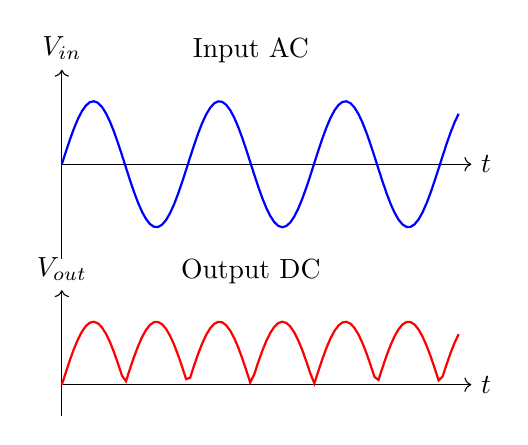
\begin{tikzpicture}[scale=0.8]
    % Input
    \draw[->] (0,0) -- (6.5,0) node[right] {\(t\)};
    \draw[->] (0,-1.5) -- (0,1.5) node[above] {\(V_{in}\)};
    \draw[blue, thick] plot[domain=0:6.3, samples=100] (\x, {sin(deg(\x) * 3.14)});
    \node at (3,1.8) {Input AC};
    
    % Output
    \begin{scope}[yshift=-3.5cm]
        \draw[->] (0,0) -- (6.5,0) node[right] {\(t\)};
        \draw[->] (0,-0.5) -- (0,1.5) node[above] {\(V_{out}\)};
        \draw[red, thick] plot[domain=0:6.3, samples=100] (\x, {abs(sin(deg(\x) * 3.14))});
        \node at (3,1.8) {Output DC};
    \end{scope}
\end{tikzpicture}
\caption{Input and Output Waveforms}
\end{figure}

\subparagraph{Advantages:}
Higher efficiency (81.2\%) and lower ripple factor (0.48) compared to half-wave rectifier.

\paragraph{Mnemonic:}
\emph{Center-Tap: Two Diodes take turns using the Middle Path.}

% ========================================
% QUESTION 2(a) OR: Concept of Capacitors (3 marks)
% Demonstrates: Definition, Formula
% ========================================

\subsection{Question 2(a) OR [3 marks]}
\textbf{Explain concept of capacitors.}

\subsubsection{Solution}
A \textbf{Capacitor} is a passive electronic component that stores electrical energy in an electric field. It consists of two conductive plates separated by an insulating material called a dielectric.

\paragraph{Key Concepts:}
\begin{itemize}
    \item \textbf{Function:} Opposes change in voltage and blocks DC while passing AC.
    \item \textbf{Capacitance (C):} The ability to store charge. Measured in Farads (F).
    \item \textbf{Formula:} \(Q = C \times V\) where Q is charge, V is voltage.
    \item \textbf{Physical Construction:} \(C = \frac{\epsilon A}{d}\) (Increases with area A, decreases with distance d).
\end{itemize}

\paragraph{Mnemonic:}
\emph{Capacitor Capacity: Stores Charge on Plates separated by Dielectric.}

% ========================================
% QUESTION 2(b) OR: Resistor Calc (4 marks)
% Demonstrates: Multiple calculations
% ========================================

\subsection{Question 2(b) OR [4 marks]}
\textbf{Calculate value of resistor and tolerance for following color bands on resistor: (1) Brown, Green, yellow, gold (2) Grey, blue, brown}

\subsubsection{Solution}
Resistor values are determined by decoding the colored bands printed on the component body. This standardization allows for easy identification of resistance and tolerance values.

\paragraph{1. Brown, Green, Yellow, Gold:}
\begin{description}
    \item[Bands:] Brown (1), Green (5), Yellow (\(\times 10^4\)), Gold (\(\pm 5\%\)).
    \item[Calculation:] First digit 1, Second digit 5, Multiplier \(10^4\).
    \[ R = 15 \times 10,000 \Omega = 150,000 \Omega = 150 k\Omega \]
    \item[Tolerance:] Gold band indicates \(\pm 5\%\).
    \item[Result:] \textbf{150 k\(\Omega\) \(\pm 5\%\)}.
\end{description}

\paragraph{2. Grey, Blue, Brown:}
\begin{description}
    \item[Bands:] Grey (8), Blue (6), Brown (\(\times 10^1\)), No Fourth Band (Default \(\pm 20\%\)).
    \item[Calculation:] First digit 8, Second digit 6, Multiplier \(10^1\).
    \[ R = 86 \times 10 \Omega = 860 \Omega \]
    \item[Tolerance:] Absence of a fourth band implies \(\pm 20\%\) tolerance.
    \item[Result:] \textbf{860 \(\Omega\) \(\pm 20\%\)}.
\end{description}

\subparagraph{Significance:}
Correctly identifying resistor values is critical for circuit stability. A tolerance of \(20\%\) means the actual value of the \(860 \Omega\) resistor could vary between \(688 \Omega\) and \(1032 \Omega\).

\paragraph{Mnemonic:}
\emph{First Two Digits \(\rightarrow\) Multiplier \(\rightarrow\) Tolerance.}

% ========================================
% QUESTION 2(c) OR: Bridge Rectifier (7 marks)
% Demonstrates: Circuit, Waveform
% ========================================

\subsection{Question 2(c) OR [7 marks]}
\textbf{Explain working of Full wave bridge rectifier with circuit diagram and wave form.}

\subsubsection{Solution}
A \textbf{Bridge Rectifier} uses four diodes in a bridge configuration to convert AC to DC without requiring a center-tapped transformer.

\paragraph{Circuit Diagram:}
\begin{figure}[H]
\centering

\begin{circuitikz}[scale=1]
    % Transformer
    \draw (0,0) node[transformer](T){};
    \node[left] at (T.A1) {AC In};
    \node[left] at (T.A2) {AC In};
    
    % Bridge Diamond Nodes
    % Left (GND ref): (2.5, 0)
    % Right (Output): (5.5, 0)
    % Top (AC1): (4, 1.5)
    % Bottom (AC2): (4, -1.5)
    
    % Connect Transformer to Bridge AC inputs
    \draw (T.B1) |- (4, 1.5);
    \draw (T.B2) |- (4, -1.5);
    
    % Diodes
    % Top -> Right (Positive Half)
    \draw (4, 1.5) to[D*, l=\(D_1\)] (5.5, 0);
    % Bottom -> Right (Negative Half)
    \draw (4, -1.5) to[D*, l=\(D_2\)] (5.5, 0);
    % Left -> Top (Return Path)
    \draw (2.5, 0) to[D*, l=\(D_4\)] (4, 1.5);
    % Left -> Bottom (Return Path)
    \draw (2.5, 0) to[D*, l=\(D_3\)] (4, -1.5);
    
    % Load Connection
    % Right (+) -> Resistor -> Ground
    \draw (5.5, 0) -- (7,0) to[R, l=\(R_L\)] (7, -2) node[ground]{};
    \draw (7, 0) -- (8,0) node[right]{+ \(V_{out}\)};
    
    % Left (-) -> Ground
    \draw (2.5, 0) node[ground]{};
    
\end{circuitikz}
\caption{Full Wave Bridge Rectifier}
\end{figure}

\paragraph{Working Principle:}
\begin{enumerate}
    \item \textbf{Positive Half Cycle:} Top terminal is positive. Diodes \(D_1\) and \(D_3\) are Forward Biased (ON). \(D_2\) and \(D_4\) are OFF. Current flows through \(D_1 \rightarrow R_L \rightarrow D_3\).
    \item \textbf{Negative Half Cycle:} Bottom terminal is positive. Diodes \(D_2\) and \(D_4\) are Forward Biased (ON). \(D_1\) and \(D_3\) are OFF. Current flows through \(D_2 \rightarrow R_L \rightarrow D_4\).
    \item \textbf{Result:} Current always flows through \(R_L\) in the same direction.
\end{enumerate}

\paragraph{Waveforms:}
\begin{figure}[H]
\centering
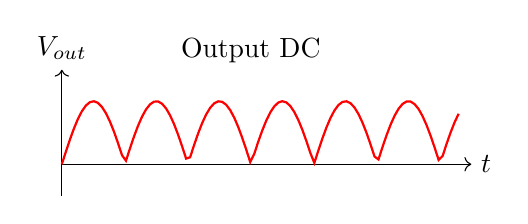
\begin{tikzpicture}[scale=0.8]
    % Output
    \draw[->] (0,0) -- (6.5,0) node[right] {\(t\)};
    \draw[->] (0,-0.5) -- (0,1.5) node[above] {\(V_{out}\)};
    \draw[red, thick] plot[domain=0:6.3, samples=100] (\x, {abs(sin(deg(\x) * 3.14))});
    \node at (3,1.8) {Output DC};
\end{tikzpicture}
\caption{Output Waveform}
\end{figure}

\subparagraph{Advantages:}
Does not require bulky center-tapped transformer. PIV rating of diodes is half that of center-tap circuit (\(V_m\) vs \(2V_m\)).

\paragraph{Mnemonic:}
\emph{Bridge Crosses Current One Way Using 4 Diodes.}

% ========================================
% QUESTION 3(a): Light Dependent Resistor (3 marks)
% Demonstrates: Definition, Principle, Symbol
% ========================================

\section{Question 3}

\subsection{Question 3(a) [3 marks]}
\textbf{Explain Light dependent resistor (LDR).}

\subsubsection{Solution}
A \textbf{Light Dependent Resistor (LDR)}, also known as a photoresistor, is a passive component whose resistance decreases as the intensity of incident light increases. It is made of high-resistance semiconductor material like Cadmium Sulfide (CdS).

\paragraph{Working Principle:}
\begin{itemize}
    \item \textbf{Darkness:} In the absence of light, LDR has very high resistance (Mega-ohms), effectively acting as an open switch.
    \item \textbf{Light:} When photons fall on the surface, electron-hole pairs are generated, increasing conductivity and drastically reducing resistance (to a few hundred ohms).
\end{itemize}

\paragraph{Symbol:}
\begin{figure}[H]
\centering
\begin{circuitikz}
    \draw (0,0) to[photoresistor, l=LDR] (2,0);
\end{circuitikz}
\caption{Symbol of LDR}
\end{figure}

\paragraph{Applications:}
Automatic street lights, camera exposure meters, and optical alarms.

\paragraph{Mnemonic:}
\emph{Light Down, Resistance Up (Dark = High R); Light Up, Resistance Down (Bright = Low R).}

% ========================================
% QUESTION 3(b): Half Wave Rectifier (4 marks)
% Demonstrates: Circuit, Waveform, Explanation
% ========================================

\subsection{Question 3(b) [4 marks]}
\textbf{Explain half wave rectifier circuit with wave form.}

\subsubsection{Solution}
A \textbf{Half Wave Rectifier} uses a single diode to convert AC voltage into pulsating DC voltage by allowing current to flow during only one half-cycle of the input.

\paragraph{Circuit Diagram:}
\begin{figure}[H]
\centering
\begin{circuitikz}[scale=1]
    \draw (0,0) to[sV, l=AC Input] (0,2) -- (2,2) to[D, l=D] (4,2) -- (4,0) to[R, l=\(R_L\)] (2,0) -- (0,0);
    \draw (2,0) node[ground]{};
    \draw (4,2) to[short, -o] (5,2) node[right]{+ \(V_{out}\)};
    \draw (4,0) to[short, -o] (5,0) node[right]{-};
\end{circuitikz}
\caption{Half Wave Rectifier Circuit}
\end{figure}

\paragraph{Operation:}
\begin{enumerate}
    \item \textbf{Positive Half Cycle:} The diode is forward biased and conducts current through the load resistor \(R_L\). Output voltage closely follows the input positive half.
    \item \textbf{Negative Half Cycle:} The diode is reverse biased and blocks current. The output voltage is zero.
\end{enumerate}

\paragraph{Waveforms:}
\begin{figure}[H]
\centering
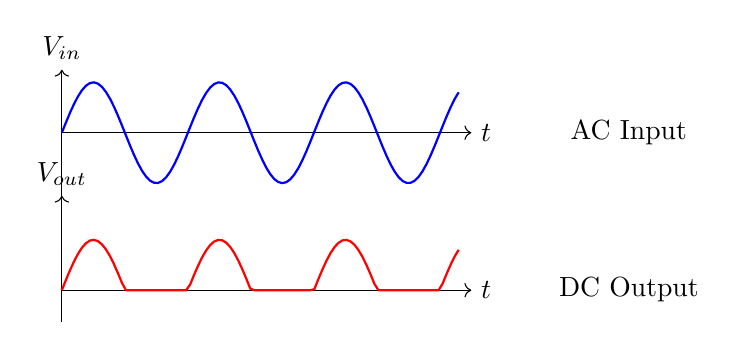
\begin{tikzpicture}[scale=0.8]
    % Input
    \draw[->] (0,2.5) -- (6.5,2.5) node[right] {\(t\)};
    \draw[->] (0,1.5) -- (0,3.5) node[above] {\(V_{in}\)};
    \draw[blue, thick] plot[domain=0:6.3, samples=100] (\x, {2.5 + 0.8*sin(deg(\x) * 3.14)});
    \node at (9,2.5) {AC Input};

    % Output
    \draw[->] (0,0) -- (6.5,0) node[right] {\(t\)};
    \draw[->] (0,-0.5) -- (0,1.5) node[above] {\(V_{out}\)};
    \draw[red, thick] plot[domain=0:6.3, samples=100] (\x, {max(0, 0.8*sin(deg(\x) * 3.14))});
    \node at (9,0) {DC Output};
\end{tikzpicture}
\caption{Input and Output Waveforms}
\end{figure}

\paragraph{Mnemonic:}
\emph{Half Wave: One Diode, One Bump per Cycle.}

% ========================================
% QUESTION 3(c): Clipper Circuits (7 marks)
% Demonstrates: List, Two types with waveforms
% ========================================

\subsection{Question 3(c) [7 marks]}
\textbf{List different types of clipper circuits and draw any two types of clipper circuits with its wave forms.}

\subsubsection{Solution}
\textbf{Clippers} are wave-shaping circuits that remove or ``clip'' a portion of the input signal without distorting the remaining part.

\paragraph{Types of Clippers:}
\begin{enumerate}
    \item Series Positive Clipper
    \item Series Negative Clipper
    \item Shunt (Parallel) Positive Clipper
    \item Shunt (Parallel) Negative Clipper
    \item Biased Clipper (Positive/Negative)
    \item Combination Clipper
\end{enumerate}

\paragraph{1. Series Positive Clipper:}
This circuit removes the positive half-cycle of the input AC signal. 
\begin{itemize}
    \item \textbf{Operation:} When the input voltage is positive, the diode is reverse biased (open circuit), and no current flows to the load. The output is zero. When the input is negative, the diode is forward biased (short circuit), and the negative half-cycle appears across the load.
\end{itemize}

\begin{figure}[H]
\centering
\begin{circuitikz}[scale=1]
    % Circuit
    \draw (0,0) to[sV, l=AC] (0,2) -- (1,2) to[D*, l=D, invert] (3,2) to[R, l=\(R_L\)] (3,0) -- (0,0);
    \draw (3,0) node[ground]{};
    \draw (3,2) to[short, -o] (4,2) node[right]{Output};
\end{circuitikz}
\caption{Series Positive Clipper}
\end{figure}

\subparagraph{Waveform:}
\begin{figure}[H]
\centering
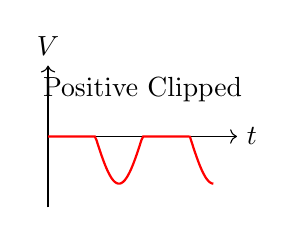
\begin{tikzpicture}[scale=0.6]
    \draw[->] (0,0) -- (4,0) node[right] {\(t\)};
    \draw[->] (0,-1.5) -- (0,1.5) node[above] {\(V\)};
    \draw[red, thick] plot[domain=0:3.5, samples=100] (\x, {min(0, sin(deg(\x)*3.14))});
    \node at (2,1) {Positive Clipped};
\end{tikzpicture}
\caption{Output of Positive Clipper}
\end{figure}

\paragraph{2. Series Negative Clipper:}
This circuit removes the negative half-cycle of the input signal.
\begin{itemize}
    \item \textbf{Operation:} During the positive half-cycle, the diode is forward biased, allowing current to flow to the load. The output follows the input. During the negative half-cycle, the diode is reverse biased, blocking current flow. The output is zero.
\end{itemize}

\begin{figure}[H]
\centering
\begin{circuitikz}[scale=1]
    % Circuit
    \draw (0,0) to[sV, l=AC] (0,2) -- (1,2) to[D*, l=D] (3,2) to[R, l=\(R_L\)] (3,0) -- (0,0);
    \draw (3,0) node[ground]{};
    \draw (3,2) to[short, -o] (4,2) node[right]{Output};
\end{circuitikz}
\caption{Series Negative Clipper}
\end{figure}

\subparagraph{Waveform:}
\begin{figure}[H]
\centering
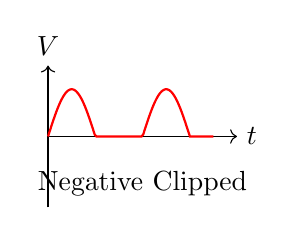
\begin{tikzpicture}[scale=0.6]
    \draw[->] (0,0) -- (4,0) node[right] {\(t\)};
    \draw[->] (0,-1.5) -- (0,1.5) node[above] {\(V\)};
    \draw[red, thick] plot[domain=0:3.5, samples=100] (\x, {max(0, sin(deg(\x)*3.14))});
    \node at (2,-1) {Negative Clipped};
\end{tikzpicture}
\caption{Output of Negative Clipper}
\end{figure}

\paragraph{Applications:}
Clippers are widely used in noise limiters, protection of sensitive circuits from voltage spikes, and modifying waveform shapes in communication systems.

\paragraph{Mnemonic:}
\emph{Series Clipper: Diode in Series with Load. Direction of Diode determines which half passes.}

% ========================================
% QUESTION 3(a) OR: Inductance (3 marks)
% Demonstrates: Definitions, Differences
% ========================================

\subsection{Question 3(a) OR [3 marks]}
\textbf{Explain self and mutual inductance in brief.}

\subsubsection{Solution}
Inductance is the property of a conductor to oppose changes in current flowing through it.

\paragraph{Self Inductance (L):}
It is the phenomenon where a changing current in a coil induces an EMF in the \textit{same} coil. This induced EMF opposes the change in current (Lenz's Law).
\begin{itemize}
    \item \textbf{Unit:} Henry (H).
    \item \textbf{Formula:} \(E = -L \frac{dI}{dt}\).
\end{itemize}

\paragraph{Mutual Inductance (M):}
It is the phenomenon where a changing current in one coil (Primary) induces an EMF in a neighboring coil (Secondary). This is the working principle of transformers.
\begin{itemize}
    \item \textbf{Coupling:} Depends on the magnetic linkage between coils.
    \item \textbf{Formula:} \(E_2 = -M \frac{dI_1}{dt}\).
\end{itemize}

\paragraph{Mnemonic:}
\emph{Self = One Coil acting on itself; Mutual = Two Coils interacting.}

% ========================================
% QUESTION 3(b) OR: Ripple Factor (4 marks)
% Demonstrates: Definitions, Formulas
% ========================================

\subsection{Question 3(b) OR [4 marks]}
\textbf{Explain the following terms in brief. (1) Ripple factor (2) Ripple frequency.}

\subsubsection{Solution}
In rectifier circuits, the output is not pure DC but contains AC components called ripples.

\paragraph{1. Ripple Factor (\texorpdfstring{\(\gamma\)}{gamma}):}
Ripple factor is a measure of the effectiveness of a rectifier in converting AC to DC. It is defined as the ratio of the RMS value of the AC component to the DC component in the output.
\begin{itemize}
    \item \textbf{Formula:} \(\gamma = \frac{V_{ac(rms)}}{V_{dc}} = \sqrt{{\left(\frac{V_{rms}}{V_{dc}}\right)}^2 - 1}\).
    \item \textbf{Values:} Half Wave = 1.21, Full Wave = 0.48. Lower is better.
\end{itemize}

\paragraph{2. Ripple Frequency (\texorpdfstring{\(f_r\)}{fr}):}
It is the frequency of the ripple voltage appearing at the output of the rectifier.
\begin{itemize}
    \item \textbf{Half Wave:} \(f_r = f_{in}\) (Fundamentals frequency same as input).
    \item \textbf{Full Wave:} \(f_r = 2 f_{in}\) (Ripple frequency is double the input).
\end{itemize}

\paragraph{Mnemonic:}
\emph{Factor = Quality (AC/DC); Frequency = Rate (Hz).}

% ========================================
% QUESTION 3(c) OR: Clamper Circuits (7 marks)
% Demonstrates: List, Two types with waveforms, Detailed
% ========================================

\subsection{Question 3(c) OR [7 marks]}
\textbf{List different types of clamper circuits and draw any two types of clamper circuits with its wave forms.}

\subsubsection{Solution}
A \textbf{Clamper Circuit} (or DC Restorer) shifts the entire signal voltage level up or down without changing the shape of the waveform. It essentially adds a DC component to the AC signal.

\paragraph{Types of Clampers:}
\begin{enumerate}
    \item Positive Clamper (Shifts signal Up)
    \item Negative Clamper (Shifts signal Down)
    \item Biased Positive Clamper
    \item Biased Negative Clamper
\end{enumerate}

\paragraph{1. Positive Clamper:}
This circuit shifts the input waveform in the positive direction such that the negative peak sits on the zero level (or reference level). 
\begin{itemize}
    \item \textbf{Mechanism:} During the negative half-cycle, the diode conducting charges the capacitor. During the positive half-cycle, the diode is off, and the capacitor voltage adds to the input voltage.
\end{itemize}

\begin{figure}[H]
\centering
\begin{circuitikz}[scale=1]
    % Circuit
    \draw (0,0) to[sV, l=AC] (0,2) to[C, l=C] (2,2) to[D*, l=D, invert] (2,0) -- (0,0);
    \draw (2,2) -- (4,2) to[R, l=\(R_L\)] (4,0) -- (2,0);
    \draw (2,0) node[ground]{};
    \draw (4,2) to[short, -o] (5,2) node[right]{Output};
\end{circuitikz}
\caption{Positive Clamper Circuit}
\end{figure}

\subparagraph{Waveform:}
\begin{figure}[H]
\centering
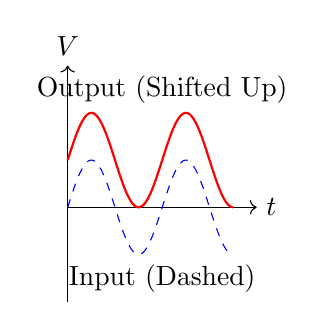
\begin{tikzpicture}[scale=0.6]
    \draw[->] (0,0) -- (4,0) node[right] {\(t\)};
    \draw[->] (0,-2) -- (0,3) node[above] {\(V\)};
    \draw[blue, dashed] plot[domain=0:3.5, samples=100] (\x, {sin(deg(\x)*3.14)});
    \draw[red, thick] plot[domain=0:3.5, samples=100] (\x, {1 + sin(deg(\x)*3.14)});
    \node at (2,2.5) {Output (Shifted Up)};
    \node at (2,-1.5) {Input (Dashed)};
\end{tikzpicture}
\caption{Input and Positive Clamped Output}
\end{figure}

\paragraph{2. Negative Clamper:}
This circuit shifts the input waveform in the negative direction such that the positive peak touches the zero level.
\begin{itemize}
    \item \textbf{Mechanism:} The diode polarity is reversed compared to the positive clamper. The capacitor charges with opposite polarity, effectively subtracting a DC voltage from the input signal.
\end{itemize}

\begin{figure}[H]
\centering
\begin{circuitikz}[scale=1]
    % Circuit
    \draw (0,0) to[sV, l=AC] (0,2) to[C, l=C] (2,2) to[D*, l=D] (2,0) -- (0,0);
    \draw (2,2) -- (4,2) to[R, l=\(R_L\)] (4,0) -- (2,0);
    \draw (2,0) node[ground]{};
    \draw (4,2) to[short, -o] (5,2) node[right]{Output};
\end{circuitikz}
\caption{Negative Clamper Circuit}
\end{figure}

\subparagraph{Waveform:}
\begin{figure}[H]
\centering
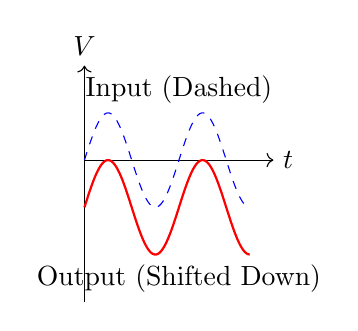
\begin{tikzpicture}[scale=0.6]
    \draw[->] (0,0) -- (4,0) node[right] {\(t\)};
    \draw[->] (0,-3) -- (0,2) node[above] {\(V\)};
    \draw[blue, dashed] plot[domain=0:3.5, samples=100] (\x, {sin(deg(\x)*3.14)});
    \draw[red, thick] plot[domain=0:3.5, samples=100] (\x, {-1 + sin(deg(\x)*3.14)});
    \node at (2,1.5) {Input (Dashed)};
    \node at (2,-2.5) {Output (Shifted Down)};
\end{tikzpicture}
\caption{Input and Negative Clamped Output}
\end{figure}

\paragraph{Mnemonic:}
\emph{Clamp Up (Positive) or Clamp Down (Negative). Capacitor holds the DC offset.}

% ========================================
% QUESTION 4(a): Symbols (3 marks)
% Demonstrates: Circuit Symbols
% ========================================

\section{Question 4}

\subsection{Question 4(a) [3 marks]}
\textbf{Draw Symbols of Zener diode, LED, and Varactor diode.}

\subsubsection{Solution}
\begin{enumerate}
    \item \textbf{Zener Diode:} Designed to operate in the reverse breakdown region. The symbol has ``bent'' cathode lines resembling the letter `Z'.
    \item \textbf{Light Emitting Diode (LED):} Emits light when forward biased. The symbol is a standard diode with arrows pointing \textit{away}, indicating light emission.
    \item \textbf{Varactor Diode:} Acts as a variable capacitor under reverse bias. The symbol includes a capacitor-like double line at the cathode.
\end{enumerate}

\paragraph{Symbols:}
\begin{figure}[H]
\centering
\begin{circuitikz}[scale=1.2]
    % Zener
    \draw (0,0) to[zDo, l=Zener, -o] (2,0);
    
    % LED
    \draw (3,0) to[leDo, l=LED, -o] (5,0);
    
    % Varactor
    \draw (6,0) to[VCo, l=Varactor, -o] (8,0);
\end{circuitikz}
\caption{Symbols of Zener, LED, and Varactor Diodes}
\end{figure}

\paragraph{Mnemonic:}
\emph{Zener is ``Z''; LED radiates Light (Arrows Out); Varactor varies like a Capacitor (Parallel plates).}

% ========================================
% QUESTION 4(b): Photodiode (4 marks)
% Demonstrates: Explanation, Working
% ========================================

\subsection{Question 4(b) [4 marks]}
\textbf{Explain Photodiode.}

\subsubsection{Solution}
A \textbf{Photodiode} is a semiconductor device that converts light energy into electrical energy (current). It is designed to operate in \textbf{Reverse Bias} condition.

\paragraph{Construction and Symbol:}
It consists of a PN junction housed in a package with a transparent window or lens to allow light to strike the junction.
\begin{figure}[H]
\centering
\begin{circuitikz}
    \draw (0,0) to[photodiode, l=Photodiode, -o] (2,0);
\end{circuitikz}
\caption{Photodiode Symbol}
\end{figure}

\paragraph{Working Principle:}
\begin{itemize}
    \item \textbf{Dark Current:} When no light falls on the reverse-biased photodiode, a very small leakage current flows due to minority carriers. This is called Dark Current.
    \item \textbf{Illumination:} When light (photons) strikes the depletion region, it breaks covalent bonds, generating electron-hole pairs.
    \item \textbf{Photocurrent:} These carriers are swept across the junction by the electric field, creating a reverse current that is linearly proportional to the intensity of incident light.
\end{itemize}

\paragraph{Applications:}
Optical communication receivers, smoke detectors, remote controls, and solar cells (in photovoltaic mode).

\paragraph{Mnemonic:}
\emph{Photo-Diode: Photons IN (Arrows In) \(\rightarrow\) Current flows (Reverse Bias).}

% ========================================
% QUESTION 4(c): Zener Diode (7 marks)
% Demonstrates: Construction, Characteristics, Working
% ========================================

\subsection{Question 4(c) [7 marks]}
\textbf{Explain construction, characteristics and working of Zener diode.}

\subsubsection{Solution}
A \textbf{Zener Diode} is a heavily doped silicon PN junction diode designed to operate in the reverse breakdown region without damage.

\paragraph{Construction:}
It is similar to a normal PN junction diode but with \textbf{heavy doping} (impurity concentration is high). This results in a very narrow depletion region along with a very strong electric field intensity. This enables the quantum tunneling effect or avalanche breakdown at specific voltages.

\paragraph{Working Principle:}
\begin{itemize}
    \item \textbf{Forward Bias:} It acts exactly like a normal diode. It starts conducting around 0.7V (for Silicon).
    \item \textbf{Reverse Bias (Pre-Breakdown):} Initially, only a small leakage current flows.
    \item \textbf{Reverse Breakdown:} When the reverse voltage reaches a specific value called the \textbf{Zener Voltage (\(V_Z\))}, the current increases sharply.
    \begin{itemize}
        \item \textbf{Zener Effect (\(< 6V\)):} Due to heavy doping, the intense electric field pulls electrons from covalent bonds (Tunneling).
        \item \textbf{Avalanche Effect (\(> 6V\)):} Accelerated minority carriers collide with atoms, knocking out more electrons (Chain reaction).
    \end{itemize}
    \item \textbf{Voltage Regulation:} In the breakdown region, the voltage across the Zener diode remains constant (\(V_Z\)) even if the current through it changes significantly.
\end{itemize}

\paragraph{V-I Characteristics:}
\begin{figure}[H]
\centering
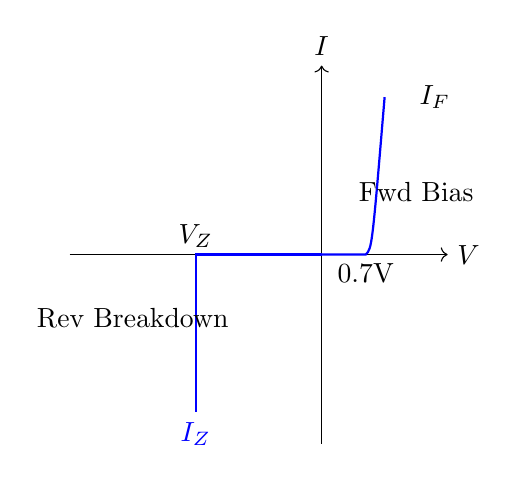
\begin{tikzpicture}[scale=0.8]
    % Axes
    \draw[->] (-4,0) -- (2,0) node[right] {\(V\)};
    \draw[->] (0,-3) -- (0,3) node[above] {\(I\)};
    
    % Forward
    % Forward
    \draw[blue, thick] (0,0) -- (0.7,0) .. controls (0.8,0.1) .. (1,2.5);
    \node[right] at (1.4, 2.5) {\(I_F\)};
    
    % Reverse
    \draw[blue, thick] (0,0) -- (-2,0) -- (-2,-2.5) node[below]{\(I_Z\)};
    
    % Labels
    \node at (0.7,-0.3) {0.7V};
    \node at (-2, 0.3) {\(V_Z\)};
    \node at (1.5, 1) {Fwd Bias};
    \node at (-3, -1) {Rev Breakdown};
    
\end{tikzpicture}
\caption{V-I Characteristics of Zener Diode}
\end{figure}

\paragraph{Mnemonic:}
\emph{Zener: Zoo for electrons in Reverse. Heavily Doped, Voltage Constant.}

% ========================================
% QUESTION 4(a) OR: Applications (3 marks)
% Demonstrates: Lists
% ========================================

\subsection{Question 4(a) OR [3 marks]}
\textbf{List applications of LED and Varactor diode.}

\subsubsection{Solution}

\paragraph{Applications of LED (Light Emitting Diode):}
\begin{enumerate}
    \item \textbf{Indicators:} widely used as power status indicators on electronic devices, computer peripherals, and traffic lights due to their long life and low power consumption.
    \item \textbf{Illumination:} Used in domestic and industrial lighting, street lights, and automotive headlamps because of their high energy efficiency and durability compared to incandescent bulbs.
    \item \textbf{Display:} They form the pixel elements in large outdoor displays, seven-segment displays for digital clocks, and backlight modules for LED TV screens.
    \item \textbf{Communication:} Infrared LEDs act as light sources in short-range optical fiber communication systems and in remote controls for televisions and AC units.
\end{enumerate}

\paragraph{Applications of Varactor Diode:}
\begin{enumerate}
    \item \textbf{Tuning Circuits:} Primarily used in the tuning stages of radio receivers and television sets to replace bulky mechanical variable capacitors. This allows for electronic tuning (Automatic Frequency Control - AFC).
    \item \textbf{Frequency Modulation (FM):} Used in FM transmitters where the audio signal modulates the diode's capacitance, thereby varying the carrier frequency.
    \item \textbf{Active Filters:} Employed in tunable active filter circuits and voltage-controlled oscillators (VCOs) to adjust the resonant frequency electronically.
    \item \textbf{Microwave Applications:} Used in parametric amplifiers and frequency multipliers (dividers) in high-frequency microwave communication circuits.
\end{enumerate}

\paragraph{Mnemonic:}
\emph{LED Lights up world; Varactor Varies Frequency (Tuning).}

% ========================================
% QUESTION 4(b) OR: Zener as Regulator (4 marks)
% Demonstrates: Circuit, Explanation
% ========================================

\subsection{Question 4(b) OR [4 marks]}
\textbf{Explain Zener diode as a voltage regulator.}

\subsubsection{Solution}
A \textbf{Voltage Regulator} maintains a constant output voltage despite changes in input voltage or load current. A Zener diode operating in the breakdown region is ideal for this purpose because its voltage (\(V_Z\)) remains constant.

\paragraph{Circuit Diagram:}
\begin{figure}[H]
\centering
\begin{circuitikz}[scale=1]
    \draw (0,0) to[sV, l=\(V_{in}\)] (0,3) to[R, l=\(R_S\)] (3,3) coordinate(top);
    \draw (top) to[zDo, l=Zener, invert] (3,0) coordinate(bot); % Reverse biased
    \draw (top) -- (5,3) to[R, l=\(R_L\)] (5,0) -- (bot);
    \draw (bot) -- (0,0);
    \draw (3,0) node[ground]{};
    \draw (5,3) to[short, -o] (6,3) node[right]{+ \(V_{out}\)};
    \draw (5,0) to[short, -o] (6,0) node[right]{-};
\end{circuitikz}
\caption{Zener Voltage Regulator}
\end{figure}

\paragraph{Working:}
\begin{enumerate}
    \item \textbf{Input Regulation (Line Regulation):} If input voltage \(V_{in}\) increases, total current increases. The Zener diode absorbs the extra current (\(I_Z\) increases), keeping the voltage drop across parallel load \(R_L\) constant at \(V_Z\). Voltage drop across \(R_S\) increases to balance the excess \(V_{in}\).
    \item \textbf{Load Regulation:} If load current \(I_L\) increases (load decreases), the Zener current \(I_Z\) decreases by the same amount, keeping total current through \(R_S\) constant. Thus, output voltage \(V_{out} = V_Z\) remains stable.
\end{enumerate}

\paragraph{Mnemonic:}
\emph{Zener absorbs the shock (Current changes) to keep Voltage steady.}

% ========================================
% QUESTION 4(c) OR: Varactor Diode (7 marks)
% Demonstrates: Construction, Working, Plot
% ========================================

\subsection{Question 4(c) OR [7 marks]}
\textbf{Explain construction, characteristics and working of Varactor diode.}

\subsubsection{Solution}
A \textbf{Varactor Diode} (or Varicap) is a variable capacitance diode that works under \textbf{reverse bias}. Measurements of its junction capacitance depend on the applied reverse voltage.

\paragraph{Construction:}
It is a PN junction diode optimized for variable capacitance.
\begin{itemize}
    \item \textbf{Junction:} The P and N regions are heavily doped to minimize series resistance.
    \item \textbf{Depletion Region:} Acts as the dielectric of a capacitor.
    \item \textbf{P and N Layers:} Act as conductive plates of the capacitor.
    \item \textbf{Package:} Encased in glass or plastic to protect the junction.
\end{itemize}

\paragraph{Working Principle:}
The Varactor diode is always operated in \textbf{reverse bias}. The basic principle is based on the variation of depletion layer width with the applied reverse voltage.
\begin{enumerate}
    \item \textbf{Depletion as Dielectric:} The depletion region allows no current to flow and acts as an insulator (dielectric) between the P-type and N-type conductive regions.
    \item \textbf{High Reverse Voltage:} When the reverse voltage (\(V_R\)) increases, the depletion layer widens. This effectively increases the distance (\(d\)) between the conductive plates. Since capacitance is inversely proportional to distance (\(C \propto \epsilon A / d\)), the junction capacitance \textbf{decreases}.
    \item \textbf{Low Reverse Voltage:} When the reverse voltage decreases, the depletion layer narrows. The distance (\(d\)) decreases, causing the junction capacitance to \textbf{increase}.
    \item \textbf{Mathematical Relationship:} The transition capacitance \(C_T\) is given by:
    \[ C_T = \frac{C(0)}{{\left(1 + \frac{V_R}{V_B}\right)}^n} \]
    Where \(C(0)\) is the zero-bias capacitance, \(V_B\) is the barrier potential (approx 0.7V for Si), and \(n\) is a doping-dependent constant (0.5 for abrupt junction). This confirms that \(C_T \propto \frac{1}{\sqrt{V_R}}\).
\end{enumerate}

\paragraph{Characteristics:}
The graph shows Capacitance (C) versus Reverse Voltage (\(V_R\)). It is a non-linear curve where C decreases as \(V_R\) increases.

\begin{figure}[H]
\centering
\begin{tikzpicture}[scale=0.8]
    \draw[->] (0,0) -- (5,0) node[right] {\(V_R\) (Reverse Voltage)};
    \draw[->] (0,0) -- (0,4) node[above] {\(C_J\) (Capacitance)};
    \draw[blue, thick] plot[domain=0.5:4.5, samples=100] (\x, {2/\x^0.5});
    \node at (3,2) {\(C \propto \frac{1}{\sqrt{V_R}}\)};
\end{tikzpicture}
\caption{C-V Characteristics of Varactor Diode}
\end{figure}

\paragraph{Mnemonic:}
\emph{Reverse Up \(\rightarrow\) Width Up \(\rightarrow\) Cap Down. (Like pulling capacitor plates apart).}

% ========================================
% QUESTION 5(a): Transistor as Switch (3 marks)
% Demonstrates: Concept, Regions
% ========================================

\section{Question 5}

\subsection{Question 5(a) [3 marks]}
\textbf{Explain transistor as a switch.}

\subsubsection{Solution}
A BJT transistor works as an electronic switch by operating in two specific regions: \textbf{Cut-off} (OFF state) and \textbf{Saturation} (ON state).

\paragraph{Operation:}
\begin{enumerate}
    \item \textbf{OFF State (Cut-off):} When the base-emitter junction is not forward-biased (Input = 0V), no collector current flows (\(I_C = 0\)). The transistor acts like an open switch. Output Voltage matches \(V_{CC}\).
    \item \textbf{ON State (Saturation):} When sufficient base current flows, the transistor conducts fully (\(V_{CE} \approx 0\)). Maximum collector current flows. It acts like a closed switch. Output Voltage is approx 0V.
\end{enumerate}

\paragraph{Mnemonic:}
\emph{Cut-off = Open (No current); Saturation = Closed (Full current).}

% ========================================
% QUESTION 5(b): CE Configuration (4 marks)
% Demonstrates: Circuit, Graph
% ========================================

\subsection{Question 5(b) [4 marks]}
\textbf{Draw Common Emitter (CE) configuration of NPN transistors and its input characteristics.}

\subsubsection{Solution}
In Common Emitter configuration, the Emitter terminal is common to both input and output.

\paragraph{Circuit Diagram:}
\begin{figure}[H]
\centering
\begin{circuitikz}[scale=1]
    % Ground to VBB to RB to Base
    \draw (0,0) node[ground]{} to[sV, l=\(V_{BB}\)] (0,2) to[R, l=\(R_B\)] (2,2) -- (2,2) node[npn, anchor=B](Q1){};
    
    % Emitter to Ground (Vertical)
    % Draw from Emitter straight down to ground level y=0
    \draw (Q1.E) -- (Q1.E |- 0,0) node[ground]{};
    
    % Collector to RC to VCC (Vertical)
    % Draw from Collector straight up
    \draw (Q1.C) -- ++(0,1) to[R, l=\(R_C\)] ++(0,2) node[vcc]{\(V_{CC}\)};
    
    % Output (Orthogonal)
    \draw (Q1.C) to[short, -o] ++(2,0) node[right]{Output (\(V_{CE}\))};
    
    % Input (Orthogonal) - Shifted to x=1.8 to avoid RB overlap
    \draw (1.8, 2) to[short, -o] (1.8, 3) node[above]{Input (\(V_{BE}\))};
\end{circuitikz}
\caption{NPN Common Emitter Configuration}
\end{figure}

\paragraph{Input Characteristics:}
It is the graph of Input Current (\(I_B\)) vs Input Voltage (\(V_{BE}\)) at constant Output Voltage (\(V_{CE}\)). It resembles a forward-biased diode curve.

\begin{figure}[H]
\centering
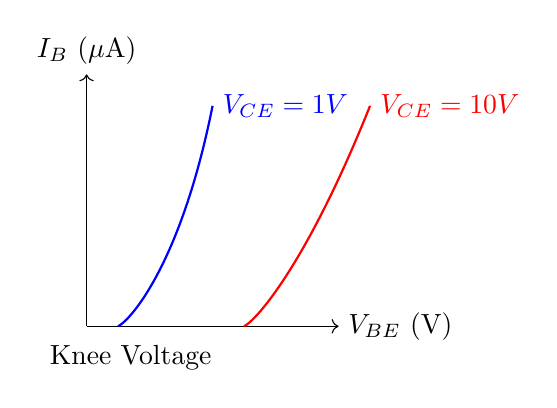
\begin{tikzpicture}[scale=0.8]
    \draw[->] (0,0) -- (4,0) node[right] {\(V_{BE}\) (V)};
    \draw[->] (0,0) -- (0,4) node[above] {\(I_B\) (\(\mu\)A)};
    \draw[blue, thick] (0.5,0) .. controls (0.7,0.1) and (1.5,1) .. (2,3.5) node[right]{\(V_{CE}=1V\)};
    \draw[red, thick] (2.5,0) .. controls (2.7,0.1) and (3.5,1) .. (4.5,3.5) node[right]{\(V_{CE}=10V\)};
    \node at (0.7,-0.5) {Knee Voltage};
\end{tikzpicture}
\caption{Input Characteristics of CE Config}
\end{figure}

\paragraph{Mnemonic:}
\emph{Input Graph is like a Diode. \(I_B\) rises after 0.7V.}

% ========================================
% QUESTION 5(c): NPN Transistor (7 marks)
% Demonstrates: Symbol, Construction, Working
% ========================================

\subsection{Question 5(c) [7 marks]}
\textbf{Draw symbol and construction of NPN Transistor and explain its working.}

\subsubsection{Solution}
An \textbf{NPN Transistor} consists of a P-type semiconductor layer sandwiched between two N-type layers.

\paragraph{Structure and Symbol:}
\begin{itemize}
    \item \textbf{Emitter (E):} Heavily doped, emits electrons.
    \item \textbf{Base (B):} Lightly doped and very thin, controls current.
    \item \textbf{Collector (C):} Moderately doped and large in size, collects electrons.
\end{itemize}

\begin{figure}[H]
\centering
\begin{circuitikz}[scale=1]
    % Symbol
    \draw (0,2) node[npn](Q){};
    \draw (Q.E) node[right]{E};
    \draw (Q.C) node[right]{C};
    \draw (Q.B) node[left]{B};
    
    % Construction Block (Widened Further)
    \draw (4,0) rectangle (11.5,3);
    \draw (6.5,0) -- (6.5,3);
    \draw (8.5,0) -- (8.5,3);
    \node at (5.25, 1.5) {N (Emit)};
    \node at (7.5, 1.5) {P (Base)};
    \node at (10, 1.5) {N (Collect)};
    \draw (5.25,0) -- (5.25,-0.5) node[below]{E};
    \draw (7.5,0) -- (7.5,-0.5) node[below]{B};
    \draw (10,0) -- (10,-0.5) node[below]{C};
\end{circuitikz}
\caption{Symbol and Construction of NPN}
\end{figure}

\paragraph{Working Principle:}
To operate as an amplifier (Active Region), the Emitter-Base junction is \textbf{Forward Biased} and Collector-Base junction is \textbf{Reverse Biased}.
\begin{enumerate}
    \item \textbf{Injection:} The forward bias (\(V_{BE}\)) causes electrons from the N-type Emitter to cross into the P-type Base.
    \item \textbf{Recombination:} Since the Base is thin and lightly doped, only a few electrons (approx 2-5\%) recombine with holes to form Base Current (\(I_B\)).
    \item \textbf{Collection:} The remaining majority of electrons (approx 95-98\%) diffuse across the base and are attracted by the high positive potential of the Collector (\(V_{CB}\)). They cross the reverse-biased junction to form Collector Current (\(I_C\)).
    \item \textbf{Equation:} The total emitter current is the sum of base and collector currents:
    \[ I_E = I_B + I_C \]
\end{enumerate}

\paragraph{Mnemonic:}
\emph{NPN = Not Pointing In (Arrow out). Emitter shoots, Base controls, Collector catches.}

% ========================================
% QUESTION 5(a) OR: Configurations Comparison (3 marks)
% Demonstrates: Table
% ========================================

\subsection{Question 5(a) OR [3 marks]}
\textbf{Compare CB, CE and CC configuration of transistor.}

\subsubsection{Solution}
\begin{table}[H]
\centering
\caption{Comparison of Transistor Configurations}
\begin{tabularx}{\textwidth}{|>{\raggedright\arraybackslash}X|>{\raggedright\arraybackslash}X|>{\raggedright\arraybackslash}X|>{\raggedright\arraybackslash}X|}
\hline
\textbf{Parameter} & \textbf{Common Base (CB)} & \textbf{Common Emitter (CE)} & \textbf{Common Collector (CC)} \\
\hline
\textbf{Input/Output} & Input: E, Output: C & Input: B, Output: C & Input: B, Output: E \\
\hline
\textbf{Input Resistance} & Very Low (\(\approx 20\Omega\)) & Medium (\(\approx 1k\Omega\)) & Very High (\(\approx 500k\Omega\)) \\
\hline
\textbf{Output Resistance} & Very High (\(\approx 1M\Omega\)) & Medium (\(\approx 40k\Omega\)) & Very Low (\(\approx 50\Omega\)) \\
\hline
\textbf{Current Gain} & Low (\(\alpha < 1\)) & High (\(\beta \approx 100\)) & High (\(\gamma \approx 100\)) \\
\hline
\textbf{Voltage Gain} & High & Medium & Low (< 1) \\
\hline
\textbf{Phase Shift} & \(0^\circ\) & \(180^\circ\) & \(0^\circ\) \\
\hline
\textbf{Application} & High Freq Applications & Audio Amplifiers & Impedance Matching \\
\hline
\end{tabularx}
\end{table}

\paragraph{Detailed Comparison:}
\begin{itemize}
    \item \textbf{Common Base (CB):} Characterized by very low input impedance and very high output impedance. It provides voltage gain but no current gain (\(\alpha < 1\)). It is primarily used for high-frequency applications and impedance matching between low sources and high loads.
    \item \textbf{Common Emitter (CE):} This is the most widely used configuration because it provides both high voltage gain and high current gain (\(\beta\)). It has moderate input and output impedance. However, it introduces a \(180^{\circ}\) phase shift between input and output signals. It is the standard for audio amplification.
    \item \textbf{Common Collector (CC):} Also known as the Emitter Follower. It has extremely high input impedance and low output impedance. It provides current gain but no voltage gain (Aux gain \(\approx 1\)). It is exclusively used for impedance matching (buffer) stages to drive low-impedance loads like speakers.
\end{itemize}

\paragraph{Mnemonic:}
\emph{CB (Base Common) = Voltage Gain; CC (Collector Common) = Current Gain (Buffer); CE (Emitter Common) = Power Gain (Best of Both).}

% ========================================
% QUESTION 5(b) OR: CE Amplifier (4 marks)
% Demonstrates: Circuit, Working
% ========================================

\subsection{Question 5(b) OR [4 marks]}
\textbf{Explain transistor as a single stage common emitter amplifier.}

\subsubsection{Solution}
A Common Emitter (CE) amplifier uses a transistor in CE configuration to amplify weak signals.

\paragraph{Circuit Diagram:}
\begin{figure}[H]
\centering
\begin{circuitikz}[scale=1]
    % Input Stage (Left)
    \draw (-2,0) node[ground]{} to[sV, l=\(V_{in}\)] (-2,2) to[C, l=\(C_{in}\)] (0,2);
    
    % Voltage Divider Bias Stage (x=0)
    % Separated from Collector path to avoid overlap
    \draw (0,2) -- (0,4.5) to[R, l=\(R_1\)] (0,6) node[vcc]{\(V_{CC}\)};
    \draw (0,2) -- (0,-0.5) to[R, l=\(R_2\)] (0,-2) node[ground]{};
    
    % Connect to Base of Transistor (x=3)
    \draw (0,2) -- (3,2) node[npn, anchor=B](Q1){};
    
    % Emitter Connections
    \draw (Q1.E) -- (Q1.E |- 0,-0.5) to[R, l=\(R_E\)] (Q1.E |- 0,-2) node[ground]{};
    % Bypass Cap
    \draw (Q1.E) -- ++(1.5,0) to[C, l=\(C_E\)] ++(0,-2) node[ground]{};
    
    % Collector Connections
    \draw (Q1.C) -- (Q1.C |- 0,4.5) to[R, l=\(R_C\)] (Q1.C |- 0,6) node[vcc]{\(V_{CC}\)};
    
    % Output
    \draw (Q1.C) to[short] ++(1.5,0) to[C, l=\(C_{out}\), -o] ++(2,0) node[right]{\(V_{out}\)};
\end{circuitikz}
\caption{Single Stage CE Amplifier}
\end{figure}

\paragraph{Working:}
\begin{enumerate}
    \item \textbf{Biasing:} Resistors \(R_1, R_2\) provide voltage divider bias to keep the transistor in the active region. \(R_E\) provides thermal stability.
    \item \textbf{Input:} The weak AC signal enters through capacitor \(C_{in}\), which blocks DC.
    \item \textbf{Amplification:} A small change in base current (\(I_b\)) causes a large change in collector current (\(I_c = \beta I_b\)). This varying current flows through \(R_C\), producing a large voltage drop (\(I_c R_C\)).
    \item \textbf{Output:} The amplified output voltage is taken across the collector, but it is \textbf{\(180^\circ\) phase shifted} relative to the input.
\end{enumerate}

\paragraph{Mnemonic:}
\emph{Weak Signal In \(\rightarrow\) Large Current Swing \(\rightarrow\) Large Voltage Drop \(\rightarrow\) Strong Signal Out (Inverted).}

% ========================================
% QUESTION 5(c) OR: CB Configuration (7 marks)
% Demonstrates: Connection, Input/Output Characteristics
% ========================================

\subsection{Question 5(c) OR [7 marks]}
\textbf{Explain common base (CB) configuration of NPN transistors with its input-output characteristics.}

\subsubsection{Solution}
In Common Base (CB) configuration, the Base terminal is grounded and common to both input and output.

\paragraph{Circuit Diagram:}
\begin{figure}[H]
\centering
\begin{circuitikz}[scale=1]
    % Transistor (Upright Standard)
    \draw (2,2) node[npn](Q){};
    
    % Base (Left -> Down -> Ground)
    \draw (Q.B) -- ++(-0.5,0) -- ++(0,-2) node[ground]{};
    
    % Emitter (Input) - Downward
    % Emitter resistor to VEE (Strictly Vertical)
    \draw (Q.E) to[R, l=\(R_E\)] ++(0,-2) to[sV, l=\(V_{EE}\)] ++(0,-1.5) node[ground]{};
    % Input Signal (Horizontal from Emitter line)
    \draw (Q.E) ++(0,-0.5) to[short, -o] ++(-2, 0) node[left]{Input (\(I_E\))};
    
    % Collector (Output) - Upward
    % Collector resistor to VCC (Strictly Vertical)
    \draw (Q.C) to[R, l=\(R_C\)] ++(0,2.5) to[sV, l=\(V_{CC}\)] ++(0,1.5) node[ground, rotate=180]{};
    % Output (Horizontal from Collector line)
    \draw (Q.C) ++(0,0.5) to[short, -o] ++(2, 0) node[right]{Output (\(V_{CB}\))};
\end{circuitikz}
\caption{Common Base Configuration}
\end{figure}

\paragraph{1. Input Characteristics:}
Graph of Input Current (\(I_E\)) vs Input Voltage (\(V_{EB}\)) at constant Output Voltage (\(V_{CB}\)).
\begin{itemize}
    \item Since the Emitter-Base junction is forward biased, the curve behaves like a normal diode. Increasing \(V_{EB}\) drastically increases \(I_E\).
    \item The effect of \(V_{CB}\) (Early Effect) is minimal but increasing \(V_{CB}\) shifts the curve slightly to the left.
\end{itemize}

\begin{figure}[H]
\centering
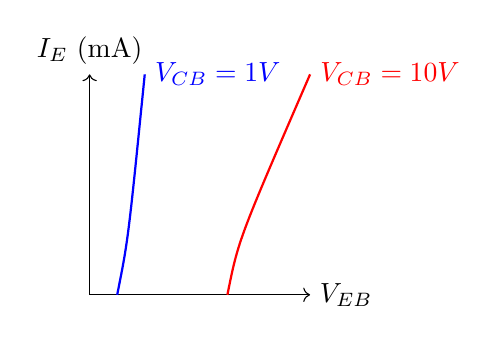
\begin{tikzpicture}[scale=0.7]
    \draw[->] (0,0) -- (4,0) node[right] {\(V_{EB}\)};
    \draw[->] (0,0) -- (0,4) node[above] {\(I_E\) (mA)};
    \draw[blue, thick] (0.5,0) .. controls (0.7,1) .. (1,4) node[right]{\(V_{CB}=1V\)};
    \draw[red, thick] (2.5,0) .. controls (2.7,1) .. (4,4) node[right]{\(V_{CB}=10V\)};
\end{tikzpicture}
\caption{CB Input Characteristics}
\end{figure}

\paragraph{2. Output Characteristics:}
Graph of Output Current (\(I_C\)) vs Output Voltage (\(V_{CB}\)) at constant Input Current (\(I_E\)).
\begin{itemize}
    \item \textbf{Active Region:} \(I_C\) is almost constant and equal to \(I_E\) (since \(\alpha \approx 1\)). It is independent of \(V_{CB}\).
    \item \textbf{Saturation Region:} When \(V_{CB}\) is negative (forward biased), \(I_C\) drops rapidly to zero.
\end{itemize}

\begin{figure}[H]
\centering
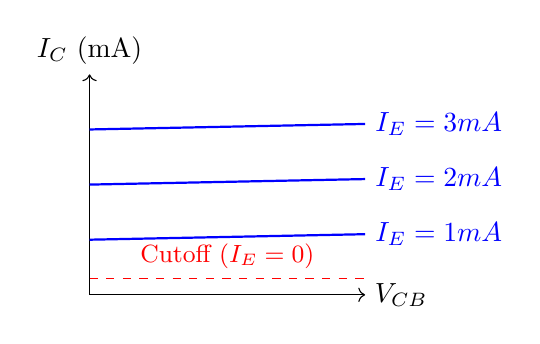
\begin{tikzpicture}[scale=0.7]
    \draw[->] (0,0) -- (5,0) node[right] {\(V_{CB}\)};
    \draw[->] (0,0) -- (0,4) node[above] {\(I_C\) (mA)};
    % Curves
    \draw[blue, thick] (0,1) -- (5,1.1) node[right]{\(I_E=1mA\)};
    \draw[blue, thick] (0,2) -- (5,2.1) node[right]{\(I_E=2mA\)};
    \draw[blue, thick] (0,3) -- (5,3.1) node[right]{\(I_E=3mA\)};
    % Cutoff
    \draw[red, dashed] (0,0.3) -- (5,0.3) node[midway, above]{\small Cutoff (\(I_E=0\))};
\end{tikzpicture}
\caption{CB Output Characteristics}
\end{figure}

\paragraph{Mnemonic:}
\emph{Common Base: Input is Emitter (Current In), Output is Collector (Current Out). Gain is Voltage, not Current.}
\end{document}
